\documentclass[nobib]{tufte-handout}

\title{Lecture 2: Eulerianity, simple graphs, and subgraphs $\cdot$ 1MA020}

\author[Vilhelm Agdur]{Vilhelm Agdur\thanks{\href{mailto:vilhelm.agdur@math.uu.se}{\nolinkurl{vilhelm.agdur@math.uu.se}}}}

\date{24 October 2023}


%\geometry{showframe} % display margins for debugging page layout

\usepackage{graphicx} % allow embedded images
  \setkeys{Gin}{width=\linewidth,totalheight=\textheight,keepaspectratio}
  \graphicspath{{graphics/}} % set of paths to search for images
\usepackage{amsmath}  % extended mathematics
\usepackage{booktabs} % book-quality tables
\usepackage{units}    % non-stacked fractions and better unit spacing
\usepackage{multicol} % multiple column layout facilities
\usepackage{lipsum}   % filler text
\usepackage{fancyvrb} % extended verbatim environments
  \fvset{fontsize=\normalsize}% default font size for fancy-verbatim environments

\usepackage{color,soul} % Highlights for text

% Standardize command font styles and environments
\newcommand{\doccmd}[1]{\texttt{\textbackslash#1}}% command name -- adds backslash automatically
\newcommand{\docopt}[1]{\ensuremath{\langle}\textrm{\textit{#1}}\ensuremath{\rangle}}% optional command argument
\newcommand{\docarg}[1]{\textrm{\textit{#1}}}% (required) command argument
\newcommand{\docenv}[1]{\textsf{#1}}% environment name
\newcommand{\docpkg}[1]{\texttt{#1}}% package name
\newcommand{\doccls}[1]{\texttt{#1}}% document class name
\newcommand{\docclsopt}[1]{\texttt{#1}}% document class option name
\newenvironment{docspec}{\begin{quote}\noindent}{\end{quote}}% command specification environment

\include{mathcommands.extratex}

\begin{document}

\maketitle% this prints the handout title, author, and date

\begin{abstract}
\noindent
We formalize the ideas we started with in the first exercise session, giving a proof of Euler's result on Eulerian circuits. We then make some more definitions about simple graphs and subgraphs, and we state some elementary results about these notions.
\end{abstract}

\section{Basic definitions, multigraphs}

The very first definition we give in this course will actually be of a \emph{multigraph}, not the simple graphs that were our first example.\sidenote[][-0.7cm]{These are of course a type of graph, so we will often just write or say ``graph'' when it is clear from context what type of graph we are referring to, or what we are saying applies to any type of graph.}

\begin{definition}
    A \emph{multigraph} $G$ is a tuple $(V, E)$, consisting of a set $V$ of \emph{vertices}, and a multiset\sidenote[][]{A multiset is just like a set, except an element may occur more than once.} $E$ of \emph{edges}. Each edge is a multiset containing two vertices from $V$, called its \emph{endpoints}. We say two vertices are \emph{adjacent} if there is an edge between them, and a vertex $v$ is \emph{incident} to an edge $e$ if $v \in e$.

    If the same edge occurs more than once in $E$, we say that these edges are \emph{parallel}. If the two endpoints of an edge are equal, we call it a \emph{loop}.

    Unless explicitly stated, we always assume that both $V$ and $E$ are finite sets. Otherwise, we say the graph is \emph{infinite}.\sidenote[][]{It may sometimes be the case that our proofs work without modification also for infinite graphs -- thinking about whether they do may be a useful thing to do when reading the proofs, to understand them better.}
\end{definition}

Next, continuing to formalize the things we learned thinking about the bridges of Königsberg, let us define what a walk is.

\begin{definition}
    Let $G = (V, E)$ be a multigraph. A \emph{walk} of length $k$ is a sequence of $k+1$ vertices $v_0 v_1 v_2\ldots v_k$ and a sequence of $k$ edges\sidenote[][]{So the length of a walk is the number of edges, not the number of vertices.} $e_1e_2\ldots e_k$ such that $e_i = \{v_{i-1}, v_i\}$ for all $i$. A \emph{trail} is a walk that uses no edge twice, and a \emph{path} is a walk that uses no vertex twice. A \emph{circuit} is a trail where the first and last vertices coincide, and a \emph{cycle} is a circuit where these are the only vertices that coincide.
\end{definition}

\begin{figure}
    \centering
    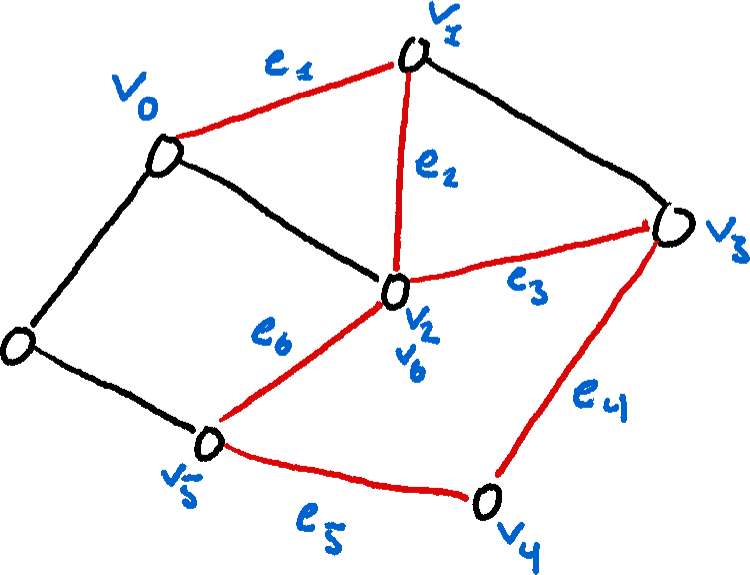
\includegraphics[width=0.7\textwidth]{graphics/L2_eulerianity_subgraphs/walk_in_graph.png}
    \caption[][0cm]{A walk in a graph, which is a trail but not a path.}
    \label{fig:walk_in_graph}
\end{figure}

We have one example of a walk in Figure \ref{fig:walk_in_graph} -- it does not repeat any of the edges, so it is a trail, but it repeats the central vertex we have labelled with both $v_2$ and $v_6$, so it is not a path.

Having introduced walks, we can give a definition of another very natural property, namely connectedness.\sidenote[][]{You've probably already seen the notion of connectedness of a subset of $\R^2$ in a calculus course, and if you've looked at other geometry it appears there as well. This is the same notion, just discretized.}

\begin{definition}
  We say that a graph $G$ is \emph{connected} if there is, for any two vertices $u, v \in G$, a walk from $u$ to $v$. We say that two vertices in a graph are connected to each other if there is a walk between them.

  Notice that there is a trivial ``lazy'' walk connecting every vertex to itself, so the relation of connectedness is an equivalence relation. The equivalence classes of this equivalence relation are called the \emph{connected components} of the graph.\sidenote[][]{We could equivalently have defined the connected components as the maximal connected subgraphs of the graph -- when we get to a formal definition of subgraph, think about why this is true.}
\end{definition}

\section{Eulerian circuits, the Bridges of Königsberg}

Let us now define the thing we were studying when we thought about the bridges of Königsberg.

\begin{definition}
  An \emph{Eulerian trail} is a trail that uses every edge in the graph exactly once -- if additionally it has the same starting and ending vertex, we call it an \emph{Eulerian circuit}. If there is an Eulerian circuit in a graph, we call the graph \emph{Eulerian}.
\end{definition}

The problem we were studying was thus to find a simple condition for when a multigraph is Eulerian. The condition we found\sidenote[][]{Hopefully.} involved the number of edges incident to a vertex, so let us also give this notion a name.

\begin{definition}
  The \emph{degree} of a vertex $v$, denoted $d_v$, is the number of edges a vertex is incident to, with loops counted twice.
\end{definition}

We now have all the language we need to formally state and prove the theorem that started graph theory all those nearly three hundred years ago.

\begin{theorem}[Euler (1736)]
  A finite connected multigraph is Eulerian if and only if all its vertices have even degree.

  \begin{proof}
    Let us begin with the easy direction of this statement: That a graph which is Eulerian will have only even-degree vertices. To see this, note that the Eulerian circuit gives us a way to pair up the edges incident to any vertex -- the path enters through one edge and leaves through another, so we pair those up. Since the circuit uses every edge, there can't be any odd edge left over in this pairing, and so the degree of the vertex can't be odd.

    So, for the harder direction, we will prove the result by induction on the number of edges.\sidenote[][]{This is a different proof than the one given in the lecture notes from last year. The reason for changing the proof is that I couldn't understand what was going on in the previous proof. Feel free to look at the other proof if this one doesn't make sense to you -- maybe it will.} The base case is $n=0$, where the graph must just be a single vertex. That this is Eulerian is trivial -- the lazy path that does nothing uses every edge in the graph, since the graph has no edges.

    Now, let $G = (V,E)$ be a finite connected multigraph with only even vertex degrees, with $n \geq 1$ edges. Pick an arbitrary vertex $v$, then pick an arbitrary edge $e = \{v, w\}$ going out from $v$.\sidenote[][]{This edge is allowed to be a loop -- think about what happens in that case.} Then pick another edge going out from $w$, making sure it hasn't already been used in our path, and so on, until you have returned to $v$. Let $W$ be the set of edges we used in this walk.

    That we will always be able to pick an unused edge to continue walking along follows from our assumption that the degrees of vertices are even -- if we were able to use an edge to get to a vertex we must also be able to pick one to leave it, since we always use up edges in pairs.
    
    \begin{figure}
      \centering
      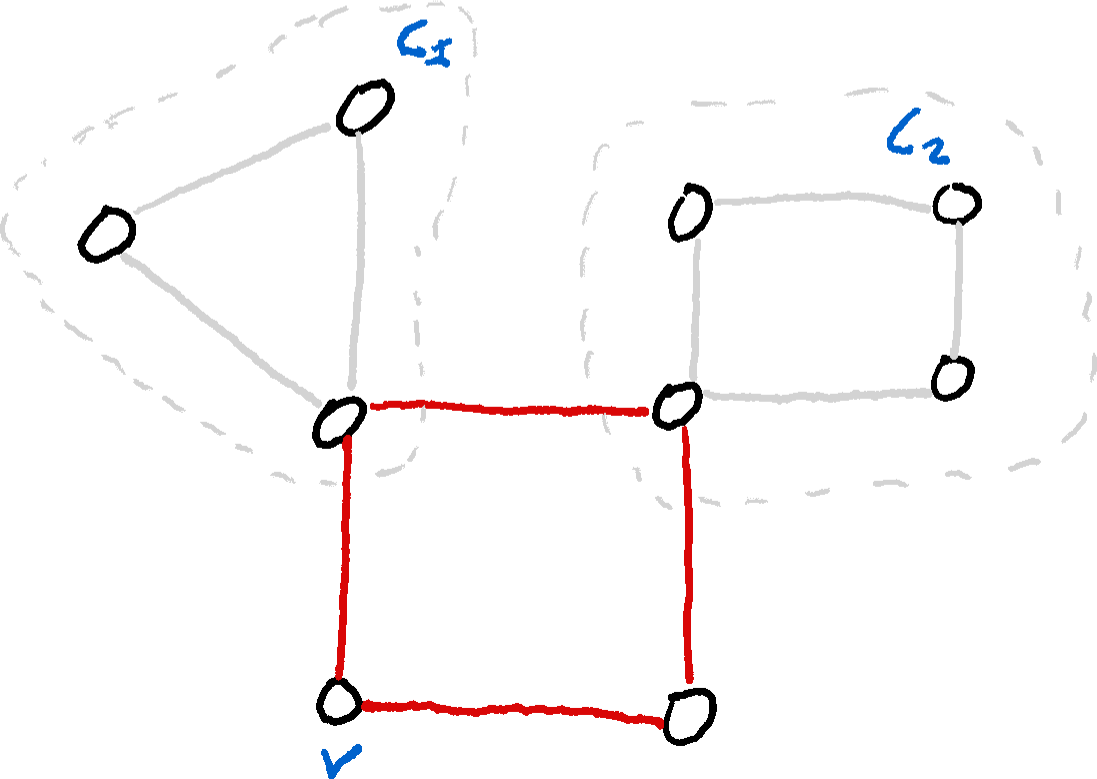
\includegraphics[width=0.7\textwidth]{graphics/L2_eulerianity_subgraphs/eulerianity_connected_components.png}
      \caption[][0cm]{A graph $G = (V,E)$ with the path $W$ highlighted in red, and the two connected components $C_1$ and $C_2$ of $H = (V, E \setminus W)$ indicated.}
      \label{fig:euler_proof_connected_components}
    \end{figure}

    Now consider the graph $H = (V, E \setminus W)$, that is, $G$ with all the edges we used in our walk removed. Let $C_1, C_2, \ldots, C_k$ be its connected components, as is illustrated in Figure \ref{fig:euler_proof_connected_components}. Now, each of these components necessarily has fewer than $n$ edges, and is of course trivially connected, so by our induction hypothesis each contains an Eulerian circuit.

    The idea now is to glue together our circuit $W$ with the circuits on the $C_i$ to get an Eulerian circuit on the entire graph. To do this, what we need is that each $C_i$ contains at least one vertex that is incident to an edge in $W$.

    To see this,\sidenote[][]{This is the hardest piece of the proof -- at least in the sense that it is hard to write in a way that is both rigorous and understandable. Once it ``clicks'' why this should be true, it is hopefully less hard. The figure, and the lecture, might help.} pick a connected component $C_i$. If $v \in C_i$, we are done, so assume it is not. We now pick some arbitrary vertex $w$ in $C_i$ -- since $G$ is by assumption connected, there exists a walk connecting $w$ to $v$. Since $v$ is not in $C_i$, this walk must at some point leave $C_i$ -- so consider the edge it leaves $C_i$ by, say, $e = \{a,b\}$, walking from $a \in C_i$ to $b \not\in C_i$. This edge must in fact be in $W$, because if it weren't, it'd be an edge of $H$, and $a$ is in $C_i$ -- and thus $b$ would also be in $C_i$, by definition of connected component, and this edge wouldn't be leaving $C_i$ at all. So the vertex $a$ must both be in $C_i$ and be incident to an edge of $W$.

    \begin{figure}
      \centering
      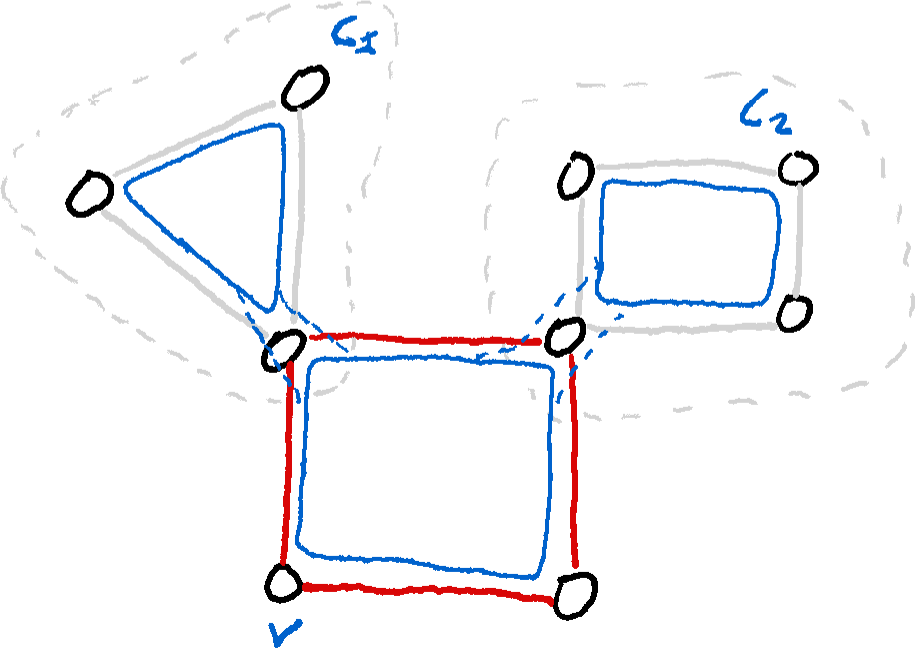
\includegraphics[width=0.7\textwidth]{graphics/L2_eulerianity_subgraphs/eulerianity_gluing_circuits.png}
      \caption[][0cm]{A graph $G = (V,E)$ with the path $W$ highlighted in red, and the two connected components $C_1$ and $C_2$ of $H = (V, E \setminus W)$ indicated. Additionally, the Eulerian circuits on the connected components and $W$ are drawn in blue, and their gluing together in dashed blue lines.}
      \label{fig:gluing_eulerian_circuits}
    \end{figure}

    So, for each $C_i$, let $a_i$ be a vertex in $C_i$ incident to an edge in $W$. We construct our Eulerian circuit on $G$ as follows: Start at $v$ and walk along $W$. Whenever you encounter an $a_i$, instead follow the Eulerian circuit in $C_i$ all the way around until you return to this $a_i$, and then proceed along $W$. That this will produce an Eulerian circuit on the entire graph should be clear, as is illustrated in Figure \ref{fig:gluing_eulerian_circuits}.
  \end{proof}
\end{theorem}

If we didn't require the trail to start and end at the same vertex, we could get away with having the start- and endpoint have odd degree. Let us state this as a corollary:

\begin{corollary}
  A finite connected graph admits an Eulerian trail if and only if either $0$ or $2$ of its vertices have odd degree.

  \begin{proof}
    If all vertices have even degree, this is just the theorem we just proved. If there are two vertices of odd degree, connect them with a new edge, so they both have even degree, and apply the theorem.
  \end{proof}
\end{corollary}

It is perhaps a bit misleading to attribute the entire theorem to Euler -- he stated it, but he only proved the easy direction. One thing he reportedly \emph{did} write a proof of is the so-called ``handshake lemma'', which also lets us settle the question of what happens if there is exactly one vertex of odd degree.

\begin{lemma}[Handshake lemma]
  Let $G = (V,E)$ be a finite graph. Then
    $$2\abs{E} = \sum_{v \in V} d_v.$$

  \begin{proof}
    To see this, we use the method of \emph{double counting} -- that is, we count one thing in two different ways. The thing we are going to count is \emph{half-edges}, that is, edges going out of vertices.\sidenote[][]{Imagine taking a pair of scissors to each edge, cutting them in half, to motivate the term. You can then recover a graph by pairing up half-edges into edges.}

    On the one hand, each edge obviously contributes two half-edges, so there are $2\abs{E}$ in the entire graph. On the other hand, each vertex contributes precisely its degree to the count of half-edges, so there are $\sum_{v\in V} d_v$ of them, proving the lemma.
  \end{proof}
\end{lemma}

\begin{corollary}
  Any graph must have an even number of odd-degree vertices.
  \begin{proof}
    The sum of the degrees must, by the handshake lemma, be even, and the sum of an odd number of odd numbers is odd.
  \end{proof}
\end{corollary}

\section{Simple graphs, basic definitions}

\begin{definition}
  A simple graph $G$ consists of a set of vertices $V$ and a set of edges $E \subseteq \binom{V}{2}$.\sidenote[][]{When $X$ is a set and $k$ is a number, the notation $\binom{X}{k}$ means the set of subsets of $X$ of size $k$. } Equivalently, it is a multigraph with no loops or parallel edges.

  So the definition we give here is actually exactly the same as what we gave for a multigraph, except wherever we said ``multiset'' there, we say ``set'' here.
\end{definition}

Since we, for a simple graph, require that there either be an edge or not, instead of having potentially many edges between two vertices, we can now actually count the number of simple graphs we can have on any given finite set.\sidenote[][]{While there are infinitely many different multigraphs even on a single vertex, of course.}

\begin{lemma}
  For any set $V$ with $n$ elements, there are $2^{\binom{n}{2}}$ different simple graphs on this set, and they all have at most $\binom{n}{2}$ edges.

  \begin{proof}
    To begin, note that
      $$\abs{\binom{V}{2}} = \binom{\abs{V}}{2} = \binom{n}{2}$$
    and so the number of subsets of $\binom{V}{2}$ is precisely $2^{\binom{n}{2}}$. Now, the edges are by definition a subset of this set, and a simple graph is determined by its vertex set and edge set, so the statement follows.

    That all the graphs have at most $\binom{n}{2}$ edges is immediate -- they are a subset of $\binom{V}{2}$, so of course a subset can't be bigger than the set it's a subset of.
  \end{proof}
\end{lemma}

Now, as we saw in the exercises in the previous session, this notion of graphs being different \emph{cares about the labels}, that is, about the underlying sets. Two graphs with different vertex sets are never equal, and even two graphs with the same vertex set that ``look equal'' can still be non-equal if we label them differently.

\begin{figure}
  \centering
  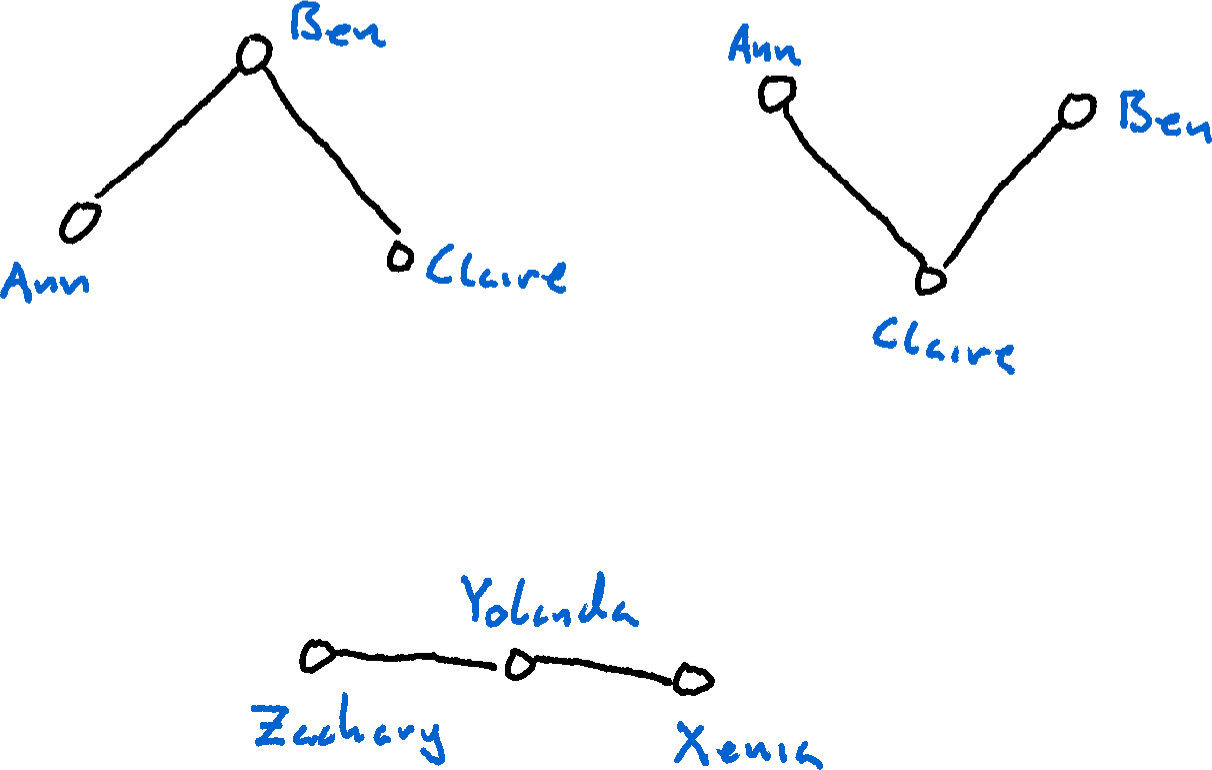
\includegraphics[width=0.7\textwidth]{graphics/L2_eulerianity_subgraphs/isomorphic_but_not_equal.png}
  \caption[][0cm]{Three non-equal but isomorphic graphs. The first two have the same underlying set but different edge-sets, the third has a different underlying set entirely.}
  \label{fig:isomorphic_but_not_equal}
\end{figure}

In some sense all three graphs in Figure \ref{fig:isomorphic_but_not_equal} are ``the same graph'' -- they are all just a line of three vertices -- but they are not the same graph in the sense of being literally equal. So we need to find a good notion of equivalence that captures this.

To do so, we start by finding what notion of functions between simple graphs is the ``right'' or ``interesting'' one.\sidenote[][]{If you want to think about morphisms between \emph{multigraphs} you have to do something slightly different.}

\begin{definition}
  Suppose $G = (V, E)$ and $H = (V', E')$ are two simple graphs. A function $f: V \to V'$ is called a \emph{graph morphism} if, whenever $\{v, w\} \in E$, we also have either $\{f(v), f(w)\} \in E'$ or $f(v) = f(w)$.\sidenote[][-0.5cm]{Whether we also allow $f(v) = f(w)$ for a graph morphism will vary a bit between texts -- I prefer this definition, but the previous year's lecture notes preferred not allowing this. So be a bit careful on the occasions where this difference actually matters!} One example of a graph morphism is given in Figure \ref{fig:graph_morphism}. 
\end{definition}

\begin{figure}
  \centering
  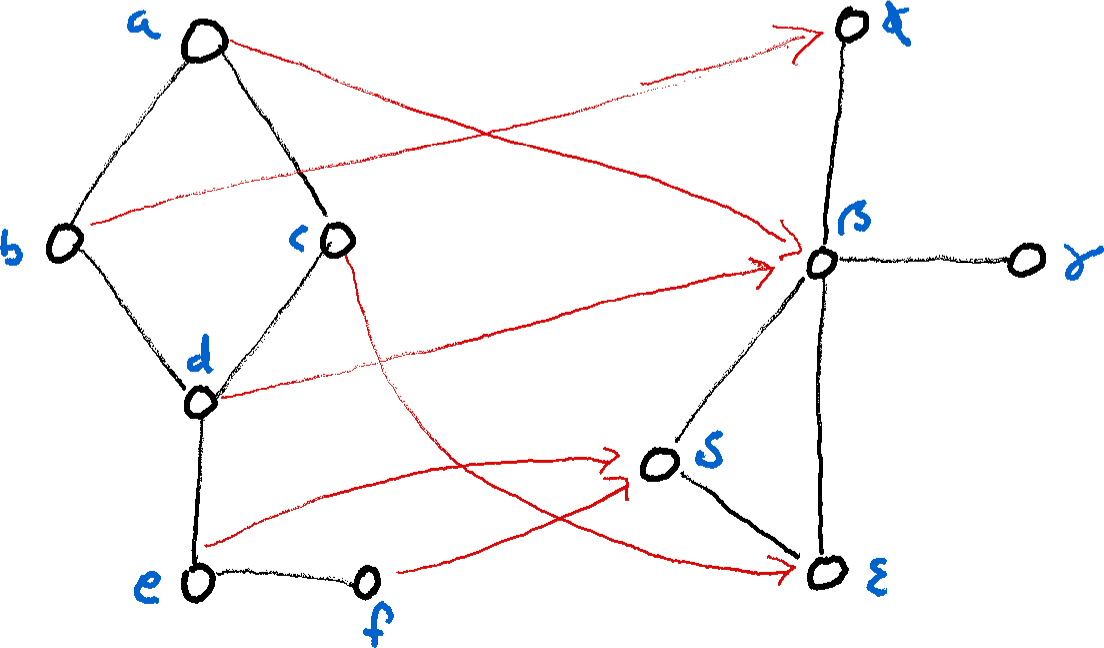
\includegraphics[width=0.7\textwidth]{graphics/L2_eulerianity_subgraphs/graph_morphism.png}
  \caption[][0.5cm]{A morphism between two graphs, one with vertices $a$ through $f$ and one with vertices $\alpha$ through $\varepsilon$. Which vertex is sent to which is illustrated with the red arrows.}
  \label{fig:graph_morphism}
\end{figure}

Note that we don't, in this definition, require that the morphism be injective -- so we are allowed to identify vertices, and since we allow $f(v) = f(w)$ we can also contract edges. Sometimes we will instead want to discuss \emph{injective} morphisms, which don't allow this. Notice that the graph in Figure \ref{fig:graph_morphism} is neither injective nor surjective.

Now that we have the notion of morphism, we can define the notion of equivalence we were looking for -- the notion of \emph{isomorphism}. As you may have seen in other courses, an isomorphism is just a bijective morphism.\sidenote[][-2cm]{The truly general definition is actually that it is a morphism that has an inverse -- so $f: G \to G'$ is an isomorphism if there exists a morphism $h: G' \to G$ such that $f \circ h$ and $h \circ f$ are the identity morphisms on the two graphs. But for graphs this is equivalent to just requiring $f$ to be bijective, and bijectivitiy is easier to think about, so we give that as our definition.}

\begin{definition}
  Two simple graphs $G$ and $H$ are isomorphic if there exists a bijective graph morphism from $G$ to $H$.
\end{definition}

The notion of isomorphism is an equivalence relation, and for each $n$ there are finitely many equivalence classes of $n$-vertex graphs.\sidenote[][]{\begin{xca}
  Prove this.
\end{xca}} This means we can finally give a definition of what we meant by the very first figure we drew in the course, the graph with no labels:

\begin{definition}
  An unlabelled simple graph is an equivalence class of simple graphs.
\end{definition}

While this definition is perhaps a bit abstract, what it means is actually rather intuitive: It means we don't care about how exactly we attach the labels or what they are, but when we actually reason about the graph we will usually have to pick a representative of the equivalence class, that is, pick one way of labelling it.

We will sometimes, in the future, be a little bit sloppy about the difference between being equal and just being isomorphic -- so for example we might say that $G$ contains $H$ when what we really mean is that $G$ has a subgraph isomorphic to $H$.

Having said this, we are of course immediately led to our last definition of this lecture, namely of what we mean by subgraph.

\begin{definition}
  A \emph{subgraph} of a graph $G = (V,E)$ is a graph $H = (V', E')$ such that $V' \subseteq V$ and $E' \subseteq E$. By how we have defined graphs, this means we also require that whenever $\{v,w\} \in E'$ we also have $v, w \in V'$.

  We will often say that a graph $H$ is a subgraph of $G$ if there exists an injective morphism from $H$ into $G$. Whenever such an injective morphism exists, there is a subgraph of $G$ that is \emph{isomorphic} to $H$,\sidenote[][]{
    \begin{xca}
      Prove this.
    \end{xca}
  } but it doesn't have to be literally equal to $H$ -- so this is an instance of us ignoring the difference between isomorphism and equality. On the few occasions the difference matters, we will be careful about it.
\end{definition}

One particular type of subgraph that is often used is the \emph{induced} subgraph.

\begin{definition}
  For any graph $G = (V, E)$ and any subset $W \subseteq V$, the \emph{induced subgraph} $G[W] = (W, E')$ has as its vertices $W$, and as its edges all the edges of $G$ with both endpoints in $W$, that is,
  $$E' = \left\{\{v, w\} \in E \given v, w \in W\right\}.$$

  So we pick all the edges we are allowed to pick given the vertices we chose.
\end{definition}

\section{Exercises}

\begin{xca}
  Suppose $G = (V, E)$ is a connected graph with four vertices of odd degree. Is it always possible to partition $E$ into two sets $E_1$ and $E_2$ so that $E = E_1 \coprod E_2$ and $(V, E_1)$ and $(V,E_2)$ admit Eulerian trails? In other words, can we colour the edges of $G$ red or blue in such a way that both the red and blue graphs contain an Eulerian trail?\sidenote[][]{This exercise is from last year's lecture notes -- I haven't thought much about it myself, so I don't know how hard it is.}

  What if we have $2k$ vertices of odd degree, for $k \geq 2$?
\end{xca}

\begin{xca}
  Suppose $f$ is a morphism from $G$ to $G'$, and $g$ is a morphism from $G'$ to $G''$. Show that $f \circ g$ is a morphism from $G$ to $G''$.\sidenote[][]{This, together with the fact that the identity function on any graph is a morphism, shows that the class of simple graphs with graph morphisms forms a \emph{category}. If you already knew what that term means, this may be somewhat interesting. If you did not, you can safely ignore this sidenote.}
\end{xca}

\begin{xca}
  Suppose $G$ and $H$ are two isomorphic graphs. Prove that $G$ is connected if and only if $H$ is, and that $G$ is Eulerian if and only if $H$ is.\sidenote[][]{For basically all notions we discuss in this course that don't obviously depend on the labelling, it will be true that they are invariant under isomorphism. These are just the two we have seen so far.}
\end{xca}

%\bibliography{references}
%\bibliographystyle{plainnat}

\end{document}
